\documentclass[a4paper,12pt]{article}
\usepackage{ amssymb }
\usepackage{mathtools}
\usepackage{amsmath}
\usepackage{amssymb}
\usepackage{listings}
\usepackage{color}
\usepackage[utf8]{inputenc}
\usepackage{amsfonts}
 \usepackage{tikz}
\DeclarePairedDelimiter\ceil{\lceil}{\rceil}
\DeclarePairedDelimiter\floor{\lfloor}{\rfloor}

\def \setB{ (0,0) circle (1cm) }
\def \setC{ (1.5,0) circle (1cm) }
\def \setA{ (60:1.5) circle (1cm) }
\def \setU { (-2, -1.5) rectangle (3.5, 2.75) }
\def \setV { (-2, -1.5) rectangle (4.0, 2.75) }
\def \setX { (-2, -1.5) rectangle (5.0, 2.75) }
  
\begin{document}

\noindent{
\framebox {
\begin{minipage}{\dimexpr\textwidth-2\fboxsep-2\fboxrule\relax}
\vspace{2mm}
1. Draw Venn diagrams that illustrate the first of the distributive laws (5.1)
\vspace{1mm}
\end{minipage}
}
}

The first distributive law is given by the expression:

\[ A \cap \left(B \cup C\right) = \left(A \cap B \right) \cup \left(A \cap C\right) \]

We can illustrate this using Venn diagrams as follows. 

\vspace{2mm}

The first sequence of diagrams illustrates $A$, $B \cup C$ and $A \cap (B \cup C)$:

\vspace{2mm}
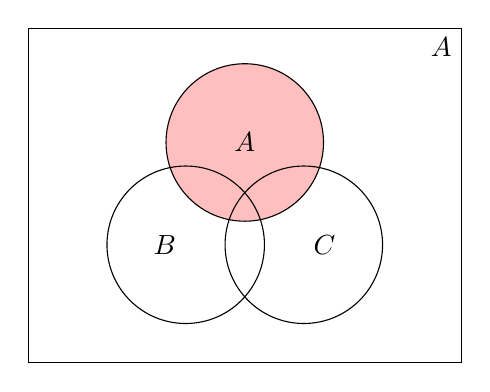
\begin{tikzpicture}
\begin{scope}
\fill[pink] \setA;
\end{scope}
\draw \setU node[below left]{$A$};
\draw \setA node {$A$};
\draw \setB node[left] {$B$};
\draw \setC node[right] {$C$};
\end{tikzpicture}

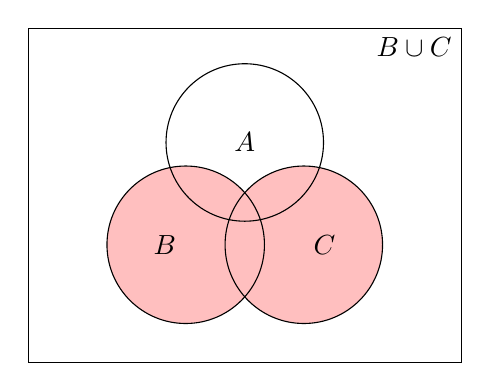
\begin{tikzpicture}
\begin{scope}
\fill[pink] \setB;
\fill[pink] \setC;
\end{scope}
\draw \setU node[below left]{$B \cup C$};
\draw \setA node {$A$};
\draw \setB node[left] {$B$};
\draw \setC node[right] {$C$};
\end{tikzpicture}

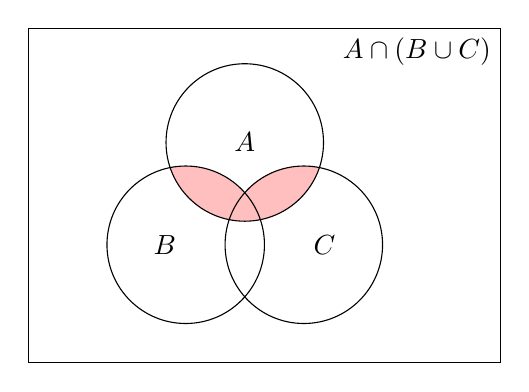
\begin{tikzpicture}
\begin{scope}
\clip \setA;
\fill[pink] \setB;
\fill[pink] \setC;
\end{scope}
\draw \setV node[below left]{$A \cap (B \cup C)$};
\draw \setA node {$A$};
\draw \setB node[left] {$B$};
\draw \setC node[right] {$C$};
\end{tikzpicture}

\newpage
The second sequence of diagrams shows $A \cap B$, $A \cap C$ and $(A \cap B) \cup (A \cap C)$:

\vspace{2mm}
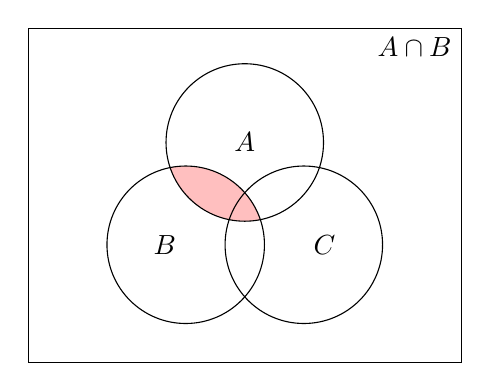
\begin{tikzpicture}
\begin{scope}
\clip \setA;
\fill[pink] \setB;
\end{scope}
\draw \setU node[below left]{$A \cap B$};
\draw \setA node {$A$};
\draw \setB node[left] {$B$};
\draw \setC node[right] {$C$};
\end{tikzpicture}

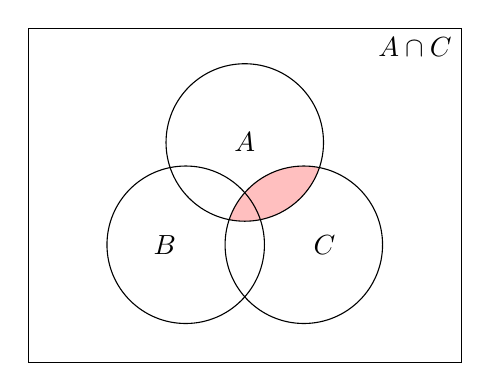
\begin{tikzpicture}
\begin{scope}
\clip \setA;
\fill[pink] \setC;
\end{scope}
\draw \setU node[below left]{$A \cap C$};
\draw \setA node {$A$};
\draw \setB node[left] {$B$};
\draw \setC node[right] {$C$};
\end{tikzpicture}

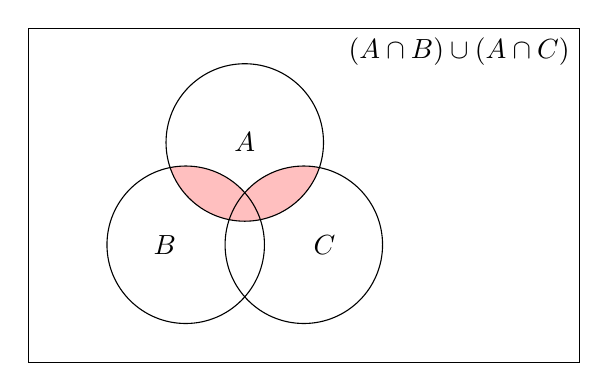
\begin{tikzpicture}
\begin{scope}
\clip \setA;
\fill[pink] \setB;
\fill[pink] \setC;
\end{scope}
\draw \setX node[below left]{$(A \cap B) \cup (A \cap C)$};
\draw \setA node {$A$};
\draw \setB node[left] {$B$};
\draw \setC node[right] {$C$};
\end{tikzpicture}

The final diagrams in each sequence are identical, hence illustrating that first distributive law $A \cap (B \cup C)= (A \cap B) \cup (A \cap C)$.

\vspace{5mm}
\noindent{
\framebox {
\begin{minipage}{\dimexpr\textwidth-2\fboxsep-2\fboxrule\relax}
\vspace{2mm}
2. Prove the generalization of DeMorgan's laws to any finite collection of sets:

\[ \overline{A_1 \cap A_2 \cap ... \cap A_n} = \overline{A_1} \cup \overline{A_2} \cup ... \cup \overline{A_n} \]
\[ \overline{A_1 \cup A_2 \cup ... \cup A_n} = \overline{A_1} \cap \overline{A_2} \cap ... \cap \overline{A_n} \]

\vspace{2mm}
\end{minipage}
}
}

We start by proving the first law, $\overline{A_1 \cap A_2 \cap ... \cap A_n} = \overline{A_1} \cup \overline{A_2} \cup ... \cup \overline{A_n}$.

\vspace{2mm}
We begin by first showing that $\overline{A_1 \cap A_2 \cap ... \cap A_n} \subseteq \overline{A_1} \cup \overline{A_2} \cup ... \cup \overline{A_n}$.

\begin{enumerate}
\item Suppose that $x \in \overline{A_1 \cap A_2 \cap ... \cap A_n}$.
\item This means that $x \notin A_1 \cap A_2 \cap ... \cap A_n$.
\item This means that $x \notin A_i$ for at least one $A_i$.
\item Hence $x \in \overline{A_i}$ for at least one $A_i$.
\item Hence we can write $x \in \overline{A_1} \cup \overline{A_2} \cup ... \cup \overline{A_n}$.
\end{enumerate}

We next show that $\overline{A_1} \cup \overline{A_2} \cup ... \cup \overline{A_n} \subseteq \overline{A_1 \cap A_2 \cap ... \cap A_n}$.

\begin{enumerate}
\item Suppose that $x \in \overline{A_1} \cup \overline{A_2} \cup ... \cup \overline{A_n}$.
\item Suppose further that $x \notin \overline{A_1 \cap A_2 \cap ... \cap A_n}$.
\item From Step $2$, it follows that $x \in A_1 \cap A_2 \cap ... \cap A_n$.
\item From Step $3$, it follows that $x \in A_i$ for all $A_i$.
\item From Step $4$, it follows that $x \notin \overline{A_i}$ for all $A_i$.
\end{enumerate}

But this raises a contradiction, since from Step 1 we must have $x \in \overline{A_i}$ for at least one $A_i$. We conclude that the presumption made at Step 2 is false, and that $x \in \overline{A_1 \cap A_2 \cap ... \cap A_n}$.

For any two sets $X$ and $Y$, we have $X=Y$ $\iff$ $X \subseteq Y$ and $Y \subseteq X$. 

We have shown here that $\overline{A_1 \cap A_2 \cap ... \cap A_n} \subseteq \overline{A_1} \cup \overline{A_2} \cup ... \cup \overline{A_n}$ and that $\overline{A_1} \cup \overline{A_2} \cup ... \cup \overline{A_n} \subseteq \overline{A_1 \cap A_2 \cap ... \cap A_n}$, so we conclude that the first of DeMorgan's laws holds true and that $\overline{A_1 \cap A_2 \cap ... \cap A_n} = \overline{A_1} \cup \overline{A_2} \cup ... \cup \overline{A_n}$.

The second law follows from the first. Set $U_i = \overline{A_i}$ for all $A_i$, so that:

\[ \overline{A_1 \cap A_2 \cap ... \cap A_n} = \overline{A_1} \cup \overline{A_2} \cup ... \cup \overline{A_n} \]
becomes

\[ \overline{ \overline{U_1} \cap \overline{U_2} \cap ... \cap \overline{U_n}} = U_1 \cup U_2 \cup ... \cup U_n \]
since $\overline{U_i} = \overline{\overline{A_i}} = A_i$.

Taking the complement of both sides, we get:

\[  \overline{U_1} \cap \overline{U_2} \cap ... \cap \overline{U_n} = \overline{U_1 \cup U_2 \cup ... \cup U_n} \]

\[   \overline{U_1 \cup U_2 \cup ... \cup U_n} = \overline{U_1} \cap \overline{U_2} \cap ... \cap \overline{U_n} \]
which establishes the result.

\noindent{
\framebox {
\begin{minipage}{\dimexpr\textwidth-2\fboxsep-2\fboxrule\relax}
\vspace{2mm}
3. Prove the generalization of equation (5.3), which is called the \textit{\textbf{principle of inclusion and exclusion}}:

\[ |A_1 \cup A_2 \cup ... \cup A_n| = |A_1| + |A_2| + ... + |A_n|  \] 
\[ - |A_1 \cap A_2| - |A_1 \cap A_3| - ... \]
\[ + |A_1 A_2 A_3| + ... \] 
\[ \vdots \]
\[ \left(-1\right)^{n-1}|A_1 \cap A_2 \cap ... \cap A_n | \]
\vspace{2mm}
\end{minipage}
}
}

We can rewrite the expression above as:

\[ \bigg|\bigcup_{i=1}^n A_i \bigg| = \sum_{i=1}^n |A_i| - \sum_{1 \le i < j \le n}|A_i \cap A_j| + ... + (-1)^{n-1}|A_1 \cap ... \cap A_n| \] 
and hence a more compact representation is given by:

\[ \bigg|\bigcup_{i=1}^n A_i \bigg| = \sum_{k=1}^n(-1)^{k+1}\left(\sum_{1 \le i_1 < ... < i_k \le n} |A_{i_1} \cap ... \cap A_{i_k}|\right) \]
or

\[ \bigg|\bigcup_{i=1}^n A_i \bigg| = \sum_{\emptyset \ne J \subseteq \{1, 2, ..., n\}}(-1)^{|J|-1} \bigg|\bigcap_{j \in J} A_j\bigg|\]

\vspace{2mm}
We proceed by induction. First consider the case $n=1$:

\[ \bigg|\bigcup_{i=1}^n A_i \bigg| = \sum_{i=1}^n |A_i|  \]

\[ \bigg|\bigcup_{i=1}^1 A_i \bigg| = \sum_{i=1}^1 |A_i|  \]

\[ |A_1| = |A_1|\]

Consider next the case $n=2$:

\[ \bigg|\bigcup_{i=1}^n A_i \bigg| = \sum_{i=1}^n |A_i|  - \sum_{1 \le i < j \le n}|A_i \cap A_j| \]

\[ \bigg|\bigcup_{i=1}^2 A_i \bigg| = \sum_{i=1}^2 |A_i|  - \sum_{1 \le i < j \le 2}|A_i \cap A_j| \]

\[ |A_1 \cup A_2| = |A_1| + |A_2| - |A_1 \cap A_2| \]

To prove this proposition, first consider the case where $A_1$ and $A_2$ are disjoint, that is, $A_1
\cap  A_2 = \emptyset$ so that $|A_1 \cap A_2| = 0$. In this case $|A_1 \cup A_2| = |A_1| + |A_2|$, which can be taken as an axiom of set theory. 

Next consider the case where $A_1 \cap A_2 \ne \emptyset$. In this case, $A_1 \cup A_2$ can be expressed as the union of two disjoint sets, $A_1$ and $\overline{A_1} \cap A_2$:

\[ A_1 \cup A_2 = A_1 \cup (\overline{A_1} \cap A_2) \]
\[ |A_1 \cup A_2| =  |A_1 \cup (\overline{A_1} \cap A_2)| \]

Since $A_1 \cap (\overline{A_1} \cap A_2) = \emptyset$, we can write:

\[ |A_1 \cup A_2| = |A_1| + |\overline{A_1} \cap A_2| \]

For any set $A$, the universe $U$ of all possible items can be represented as the union of $A$ with its complement $\overline{A}$, i.e., $U = A \cup \overline{A}$, with $A \cap \overline{A} = \emptyset$. The intersection of the universe $U$ with any set is just that set, i.e., $U \cap A = A$. 

We can reason as follows:

\[ U = A_1 \cup \overline{A_1} \]

\[ A_2 = U \cap A_2 = (A_1 \cup \overline{A_1}) \cap A_2 \]

Hence by the distribution property, $A_2$ can be written as the union of two disjoint sets:

\[ A_2 = (A_1 \cap A_2) \cup (\overline{A_1} \cap A_2) \]

Since these sets are disjoint, we can write:

\[ |A_2| = |A_1 \cap A_2| + |\overline{A_1} \cap A_2| \]

\[ |\overline{A_1} \cap A_2 | = |A_2| - |A_1 \cap A_2| \]

Substituting this into the expression above, we have:

\[ |A_1 \cup A_2| = |A_1| + |A_2| - |A_1 \cap A_2| \]

We have established the principle of inclusion and exclusion for $n=1$ and $n=2$. Proceeding by induction, suppose that the principle is true for $n$. We wish to show that it must also hold true for $n+1$.

We begin with the expression for $n$:

\[ \bigg|\bigcup_{i=1}^n A_i \bigg| = \sum_{k=1}^n(-1)^{k+1}\left(\sum_{1 \le i_1 < ... < i_k \le n} |A_{i_1} \cap ... \cap A_{i_k}|\right) \]
and note that by associativity we can write:

\[ \bigg|\bigcup_{i=1}^{n+1} A_i \bigg| = \bigg| \left(\bigcup_{i=1}^n A_i\right) \cup A_{n+1} \bigg| \]

Since $|X \cup Y| = |X| + |Y| - |X \cap Y|$ we can write:

\[  \bigg|\bigcup_{i=1}^{n+1} A_i \bigg|  = \bigg| \bigcup_{i=1}^n A_i \bigg|  + \bigg|A_{n+1}\bigg| - \bigg| \left(\bigcup_{i=1}^n A_i\right) \cap A_{n+1}  \bigg| \]

Consider the final term $|\left(\cup_{i=1}^n A_i\right) \cap A_{n+1} |$. Since intersection distributes over union, we can write:

\[ \bigg| \left(\bigcup_{i=1}^n A_i\right) \cap A_{n+1}  \bigg| = \bigg| \bigcup_{i=1}^n \left(A_i \cap A_{n+1}\right) \bigg|\]

We can now apply the induction hypothesis to this term:

\[  \bigg| \bigcup_{i=1}^n \left(A_i \cap A_{n+1}\right) \bigg| = \sum_{k=1}^n(-1)^{k+1}\left(\sum_{1 \le i_1 < ... < i_k \le n} |A_{i_1} \cap ... \cap A_{i_k} \cap A_{n+1}|\right) \]

Similarly, the first term $|\bigcup_{i=1}^n A_i|$ can be expressed in terms of the induction hypothesis:

\[   \bigg| \bigcup_{i=1}^n A_i \bigg| = \sum_{k=1}^n(-1)^{k+1}\left(\sum_{1 \le i_1 < ... < i_k \le n} |A_{i_1} \cap ... \cap A_{i_k}|\right) \]

\[ = \sum_{i_1=1}^n |A_{i_1}| + \sum_{k=2}^n \left(-1\right)^{k+1} \left(\sum_{i \le i_1 < ... < i_k \le n} |A_{i_1} \cap ... \cap A_{i_k} |\right)\]

So that $|\bigcup_{i=1}^nA_i| + |A_{n+1}|$ can be expressed as:

\[ \bigg|\bigcup_{i=1}^n A_i\bigg| + \bigg|A_{n+1}\bigg| = \sum_{i_1=1}^{n+1} |A_{i_1}| + \sum_{k=2}^n \left(-1\right)^{k+1} \left(\sum_{1 \le i_1 < ... < i_k \le n} |A_{i_1} \cap ... \cap A_{i_k} |\right) \]

For the sake of clarity, let's define the symbol $X$ to represent the second term in this expansion:

\[ X = \sum_{k=2}^n (-1)^{k+1} \left(\sum_{1 \le i_1 < ... < i_k \le n} |A_{i_1} \cap ... \cap A_{i_k}| \right) \]
and we'll use the symbol $X(k)$ to represent the $k$-th set of expressions in this expansion, for example:

\[ X(k=2) = -\{|A_1 \cap A_2| + |A_1 \cap A_3| + ... + |A_1 \cap A_n| + \]
\[ ... + |A_2 \cap A_3| + |A_2 \cap A_4| + ... + |A_2 \cap A_n| + \]
\[ ... + |A_{n-1} \cap A_n| \} \]

Similarly, we can use the symbol $Y$ to represent the expression:

\[ Y =  \sum_{k=1}^n(-1)^{k+1}\left(\sum_{1 \le i_1 < ... < i_k \le n} |A_{i_1} \cap ... \cap A_{i_k} \cap A_{n+1}|\right) \]
and we can use the symbol $Y(k)$ to represent the $k$-th set of expressions in this expansion, for example:

\[ Y(k=1) = |A_1 \cap A_{n+1}| + |A_2 \cap A_{n+1}| + ... + |A_n \cap A_{n+1}| \]

This symbolic representation allows us to combine these expressions pairwise. For example we can now write:

\[ X(k=2) - Y(k=1) = (-1) \cdot \left(\sum_{1 \le i < j \le {n+1}} |A_i \cap A_j| \right) \]

If we proceed in this same manner, combining $X(n)$ pairwise with $-Y(n-1)$, and then finally subtracting the term $Y(n)$ from the total, we express the full combination $X-Y$ as:

\[ X-Y = \sum_{k=2}^{n+1} (-1)^{k+1} \left(\sum_{1 \le i_1 < ... < i_k \le {n+1}} |A_{i_1} \cap ... \cap A_{i_k}| \right) \]

Combining all these results together, we can write:

\[ \bigg| \bigcup_{i=1}^{n+1}{A} \bigg| = \sum_{k=1}^{n+1} (-1)^{k+1} \left(\sum_{1 \le i_1 < ... < i_k \le {n+1}} |A_{i_1} \cap ... \cap A_{i_k}| \right) \]
which was the result to be proved.

\vspace{5mm}
\noindent{
\framebox {
\begin{minipage}{\dimexpr\textwidth-2\fboxsep-2\fboxrule\relax}
\vspace{2mm}
4. Show that the set of odd natural numbers is countable. 
\vspace{2mm}
\end{minipage}
}
}

An infinite set is countable if it can be put into one-to-one correspondence with the natural numbers $\mathbb{N} = \{0, 1, 2, ... \}$.

Define a one-to-one function $f(n)$ on the natural numbers $\mathbb{N}$ such that:

\[ f(n) = 2n + 1 \]

Applying this function to the natural numbers, we generate the set of odd natural numbers: 

\[ f(\mathbb{N}) = \{1, 3, 5, ...\} = \mathbb{N}_{odd} \]
The function $f$ defines a one-to-one correspondence between its range and domain, hence the set of odd natural numbers is countable.

\vspace{5mm}
\noindent{
\framebox {
\begin{minipage}{\dimexpr\textwidth-2\fboxsep-2\fboxrule\relax}
\vspace{2mm}
5. Show that for any finite set $S$, the power set $2^S$ has $2^{|S|}$ elements (that is, there are $2^{|S|}$ distinct subsets of $S$).
\vspace{2mm}
\end{minipage}
}
}

Consider first the empty set, $S = \{ \emptyset \}$. The empty set has no elements, so $|S| = 0$. The power set of the empty set consists, by definition, of (a) the empty set itself; and (b) all proper subsets of the empty set.

But the only subset of the empty set is the empty set itself, so the empty set is its own subset, and the empty set has no proper subsets (i.e., no subsets other than itself). The power set of the empty set can thus be expressed as:

\[ 2^S = \{ \{ \emptyset \}, \{ \emptyset \} \}  = \{ \{ \emptyset \} \} \]

\noindent
since a set contains no repeated elements. The cardinality of this power set is $1 = 2^0  = 2^{|S|}$, which establishes the result. 

Consider next a set with one element, $S = \{a\}$. This set has one element, so $|S| = 1$, and the power set contains two elements:

\[ 2^S = \{ \{ \emptyset \},\{a\}\} \]

\noindent
The cardinality of this power set is $2 = 2^1 = 2^{|S|}$, which establishes the result. 

Now suppose that by induction, the result is established for a set containing $n$ elements, so that if the set $S$ contains $n$ elements:

\[ S = \{a_1, a_2, ..., a_n \} \]

\noindent
with $|S| = n$, we have that the cardinality of the power set of $S$ is $2^{|S|}$.

Consider the set $S'$ containing $n+1$ elements: 

\[ S' = S  \cup \{a_{n_1}\} = \{a_1, a_2, ..., a_{n+1} \} \]

The power set of $S'$ will consist of (a) all subsets of $S$, without adjoining $a_{n+1}$, plus (b) all subsets of $S$, with $a_{n+1}$ adjoined to each subset. 

Counting (a), the set of all subsets of $S$, is just the power set of $S$ and by the induction hypothesis contains $2^n$ elements. Counting (b), the set of all subsets of $S$ with the element $a_{n+1}$ adjoined to each subset, must also contain $2^n$ elements. 

The total number of elements in the power set of $S'$ must therefore be:

\[ 2^n + 2^n = 2 \cdot 2^n = 2^{n+1} = 2^{|S'|} \]

\noindent
which establishes the result. $\square$

\vspace{2mm}
This result can be established using combinatorics as well. To construct the power set of $S$, where $|S| = n$, we start by selecting the subset that contains $0$ elements, i.e., the empty set. There is exactly $\binom{n}{0} = 1$ such subset. Next we enumerate all the $1$-subsets of $S$ by selecting all the subsets that contain exactly 1 element. There are exactly $\binom{n}{1} = n$ such subsets. To enumerate all the $2$-subsets of $S$, we select all the subsets that contain exactly 2 elements. There are exactly $\binom{n}{2}$ such subsets. 

We continue accordingly, until we finally generate the set $S$ itself by selecting the subset that contains all $n$ elements. There is exactly $\binom{n}{n} = 1$ such subset. Thus the cardinality of the power set of $S$ is given by the expression:

\[ \binom{n}{0} + \binom{n}{1} + ... + \binom{n}{n} = \sum_{k=0}^n \binom{n}{k} \]

This expression can be simplified using the Binomial Theorem:

\[ \left(x+y\right)^n = \sum_{k=0}^n \binom{n}{k}x^ky^{n-k} \]

Setting $x=1$ and $y=1$ in this expression gives:

\[ 2^n = \sum_{k=0}^n \binom{n}{k} \]

\noindent
as the cardinality of the power set of $S$, which is the desired result.

\vspace{5mm}
\noindent{
\framebox {
\begin{minipage}{\dimexpr\textwidth-2\fboxsep-2\fboxrule\relax}
\vspace{2mm}
6. Give an inductive definition for an $n$-tuple by extending the set-theoretic definition for an ordered pair.
\vspace{2mm}
\end{minipage}
}
}

An ordered pair of two elements $a$ and $b$ is denoted $(a,b)$ and can be defined in terms of set theory as the set $(a,b) = \{a, \{a,b\}\}$. 

Following this same pattern, we can define a 3-tuple as:

\[ (a,b,c) = ((a,b),c) \]
\[ = \{ (a,b), \{(a,b), c\}\}\]
\[ = \{ \{a, \{a,b\}\}, \{ \{a, \{ a,b\}\}, c\}\}\]

Given an $(n-1)$-tuple, an $n$-tuple can be defined recursively as:

\[ (a_1, a_2, ..., a_n) = ((a_1, a_2, ..., a_{n-1}),a_n) \]

\end{document}